% ================================================================
%  CHAPTER 4 - RELEASE 1: PLATFORM SECURITY & CORE ORCHESTRATION
% ================================================================
\chapter{Release 1: Platform Security \& Core Orchestration}

\section{Introduction}

The first major milestone of this project was to establish the foundational security perimeter and the core AI orchestration engine. Before we could even think about advanced governance or complex data policies, we needed to ensure two things: first, that every single request entering the platform is cryptographically authenticated at the network edge, and second, that our backend can intelligently route and stream AI workloads without bottlenecking. 

This chapter details the work completed during the first release, which spans two sprints. We cover the deployment of the edge security layer, the integration of Keycloak for identity management, and the construction of the full AI streaming pipeline using FastAPI.

% ──────────────────────────────────────────────────────────────────
\section{Release 1 Plan}
% ──────────────────────────────────────────────────────────────────

We structured the development plan for Release 1 around the most critical building blocks of the platform:

\begin{enumerate}
    \item \textbf{Sprint 1: Platform Security Entry Layer} - The focus here was establishing a strict zero-trust perimeter. We deployed Kong Gateway, enabled WAF protection, integrated Keycloak for OAuth 2.0 PKCE authentication, and configured JWT validation plugins to act as the first line of defense.
    
    \item \textbf{Sprint 2: Core Orchestration Engine} - With the gates secured, we built the actual brain of the platform. This involved developing the FastAPI backend, implementing NLP-based intent classification to route prompts dynamically, and building the token-by-token SSE streaming engine connected to Ollama.
\end{enumerate}

By knocking out these fundamental areas early, we created a secure sandbox and a fully functional AI pipeline. This gave us the stable foundation needed to focus on governance and security hardening in the subsequent releases.

% ──────────────────────────────────────────────────────────────────
\section{Release 1 Backlog}
% ──────────────────────────────────────────────────────────────────

The following table outlines the specific backlog items we identified and completed for Release 1.

\begin{table}[H]
\centering
\renewcommand{\arraystretch}{1.3}
\footnotesize
\begin{tabularx}{\textwidth}{| >{\raggedright\arraybackslash}p{3.5cm} | c | >{\raggedright\arraybackslash}X | c |}
\hline
\rowcolor{rowgray}
\textbf{Feature} & \textbf{ID} & \textbf{User Stories} & \textbf{Priority} \\
\hline
Infrastructure Deployment & 1 & As an operator, I want to deploy all services with a single command. & + + + \\
\hline
Kong Configuration & 2 & As an operator, I want Kong routes configured via decK. & + + + \\
\hline
WAF Protection & 3 & As a security engineer, I want OWASP WAF at the edge. & + + + \\
\hline
Network Security & 4 & As a security engineer, I want TLS and network segmentation. & + + \\
\hline
Logging & 5 & As an operator, I want a Kong logging plugin. & + + + \\
\hline
Authentication & 6 & As a user, I want to log in via Keycloak SSO. & + + + \\
\hline
JWT Middleware & 7 & As a developer, I want JWT middleware rejecting invalid tokens. & + + + \\
\hline
Tenant Enforcement & 8 & As a security engineer, I want tenant ID enforced from JWT. & + + + \\
\hline
ACL Management & 9 & As an admin, I want tenant-service ACLs. & + + \\
\hline
Audit Logging & 10 & As a developer, I want permission audit logs. & + + \\
\hline
Backend Core & 11 & As a developer, I want a FastAPI backend with Pydantic validation. & + + + \\
\hline
Intent Classification & 12 & As a developer, I want NLP-based intent classification. & + + + \\
\hline
Intent Cache & 13 & As a developer, I want a hot-reloadable intent cache. & + + \\
\hline
Database Models & 14 & As a developer, I want database models for requests and services. & + + + \\
\hline
Auto Schema & 15 & As a developer, I want auto-creation of tables on startup. & + + \\
\hline
Deterministic Routing & 16 & As a user, I want deterministic routing to one AI service. & + + + \\
\hline
SSE Streaming & 17 & As a user, I want token-by-token SSE streaming. & + + + \\
\hline
Ollama Client & 18 & As a developer, I want an Ollama client with error recovery. & + + + \\
\hline
Lifecycle Tracking & 19 & As a developer, I want request lifecycle tracking. & + + \\
\hline
\end{tabularx}
\caption{Release 1 Backlog}
\label{tab:release1_backlog}
\end{table}


% ══════════════════════════════════════════════════════════════════
%  SPRINT 1: PLATFORM SECURITY ENTRY LAYER
% ══════════════════════════════════════════════════════════════════
\section{Sprint 1: Platform Security Entry Layer}

The primary goal of our first sprint was to establish a zero-trust security perimeter. We needed a system that could cryptographically validate every incoming request before it ever had the chance to touch our backend logic. To achieve this, we focused on deploying Kong Gateway, integrating Keycloak, and enforcing security strictly through gateway plugins.

\begin{table}[H]
\centering
\renewcommand{\arraystretch}{1.3}
\footnotesize
\begin{tabularx}{\textwidth}{| >{\raggedright\arraybackslash}p{3.5cm} | c | >{\raggedright\arraybackslash}X | c |}
\hline
\rowcolor{rowgray}
\textbf{Feature} & \textbf{ID} & \textbf{User Stories} & \textbf{Priority} \\
\hline
Infrastructure Deployment & 1 & As an operator, I want to deploy all services with a single command. & + + + \\
\hline
Kong Configuration & 2 & As an operator, I want Kong routes configured via decK. & + + + \\
\hline
WAF Protection & 3 & As a security engineer, I want OWASP WAF at the edge. & + + + \\
\hline
Network Security & 4 & As a security engineer, I want TLS and network segmentation. & + + \\
\hline
Logging & 5 & As an operator, I want a Kong logging plugin. & + + + \\
\hline
Authentication & 6 & As a user, I want to log in via Keycloak SSO. & + + + \\
\hline
JWT Middleware & 7 & As a developer, I want JWT middleware rejecting invalid tokens. & + + + \\
\hline
Tenant Enforcement & 8 & As a security engineer, I want tenant ID enforced from JWT. & + + + \\
\hline
ACL Management & 9 & As an admin, I want tenant-service ACLs. & + + \\
\hline
Audit Logging & 10 & As a developer, I want permission audit logs. & + + \\
\hline
\end{tabularx}
\caption{Sprint 1 Backlog}
\label{tab:sprint1_backlog}
\end{table}

\subsection{Software Design}

Securing the platform meant we needed a rock-solid authentication system capable of issuing deterministic, verifiable identities. Rather than cluttering the FastAPI backend with complex security logic, we made a strategic architectural decision: externalize all security checks to the API Gateway. We selected Keycloak as our identity broker and configured it to work seamlessly with Kong Gateway to form an impenetrable perimeter.

\subsubsection{Static View: Plugin Security Pipeline}

\begin{figure}[H]
    \centering
    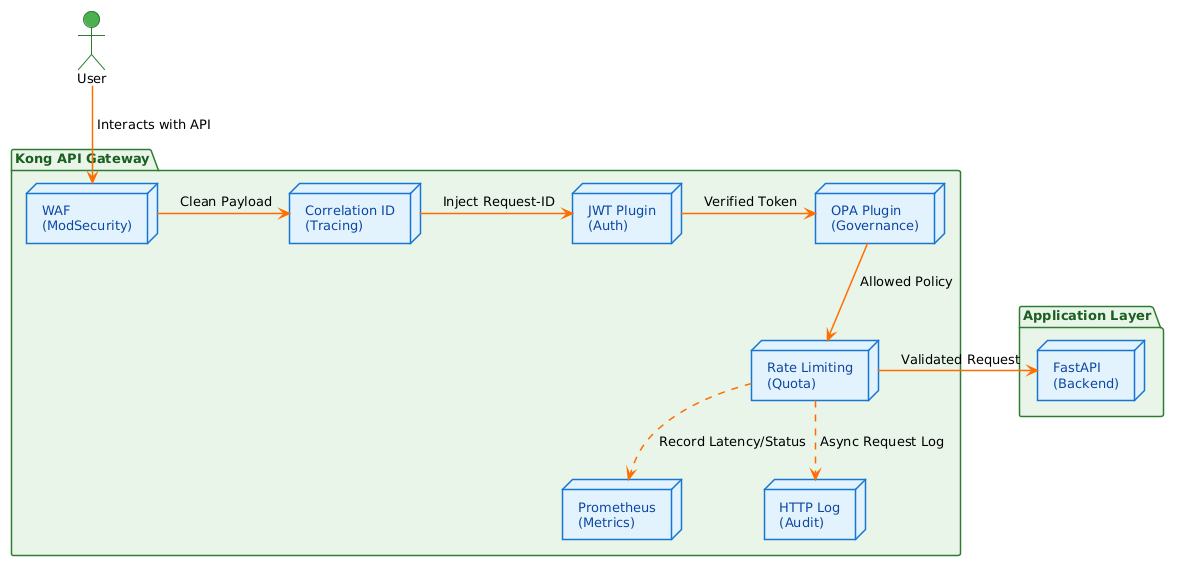
\includegraphics[width=1\textwidth]{images/plugin_pipeline_styled.png}
    \caption{Zero-Trust Kong Plugin Security Pipeline}
    \label{fig:plugin_pipeline}
\end{figure}

As shown in the pipeline above, we stacked an extensive suite of plugins directly at the gateway layer—WAF for threat detection, Correlation-IDs for tracing, JWT for authentication, OPA for governance, and Redis for rate limiting. By doing this, we guarantee that the FastAPI backend only processes requests that are 100\% verified, traceable, and authorized. 

\subsubsection{Keycloak and OAuth 2.0 PKCE}

For identity management, Keycloak handles Single Sign-On (SSO) via the OpenID Connect (OIDC) protocol. It runs atop its own dedicated PostgreSQL database and issues RS256-signed JSON Web Tokens (JWTs). To maximize security, especially for frontend client applications, we implemented the OAuth 2.0 Authorization Code flow with Proof Key for Code Exchange (PKCE).

PKCE is a massive upgrade over traditional authorization flows. It introduces a dynamic, per-request secret (the \texttt{code\_verifier} and its hash, the \texttt{code\_challenge}). By strictly enforcing this at the edge, we completely eliminate the risk of authorization code interception and Cross-Site Request Forgery (CSRF) attacks. Even if an attacker somehow intercepts the authorization code, it is mathematically useless without the original verifier.

\subsubsection{Dynamic View: Authentication Sequence Diagram}

Instead of forcing the FastAPI application to manually decrypt and validate tokens, we leverage Kong's native \textbf{JWT Plugin}. This ensures that unauthenticated traffic is dropped at the network edge, keeping the backend completely shielded.

\begin{figure}[H]
    \centering
    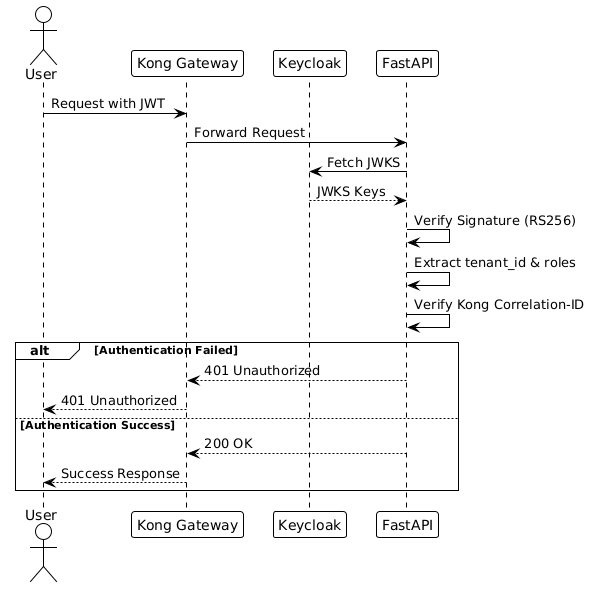
\includegraphics[width=0.85\textwidth]{images/sprint1_sequence.png}
    \caption{Authentication and Plugin-Based Request Validation Sequence}
    \label{fig:auth_sequence}
\end{figure}

The interaction flow works like this:
\begin{enumerate}
    \item The client application logs in and retrieves a secure JWT from Keycloak.
    \item The client attaches this JWT as a \texttt{Bearer} token and sends its AI request to the Kong Gateway.
    \item The \textbf{Kong JWT Plugin} intercepts the request. It uses Keycloak's public JSON Web Key Set (JWKS) to mathematically verify the RS256 signature natively, without needing to make a network call back to Keycloak.
    \item If the token is valid, Kong securely injects the \texttt{tenant\_id} and user roles into the HTTP headers and forwards the traffic to the backend. If the signature is invalid or expired, Kong instantly drops the connection with a \texttt{401 Unauthorized} status.
\end{enumerate}

This "Identity Propagation" approach is the core of our Zero-Trust architecture. Because the token is mathematically verified at the edge, the FastAPI backend implicitly trusts the upstream headers injected by Kong. This results in a highly optimized, heavily protected environment.

\subsection{Showcase}

The following figures demonstrate the successful implementation of the Zero-Trust security perimeter.

\begin{figure}[H]
    \centering
    \includegraphics[width=0.85\textwidth]{images/keycloak_login.png}
    \caption{Keycloak unified login portal intercepting unauthenticated traffic at the edge.}
    \label{fig:keycloak_login}
\end{figure}

\begin{figure}[H]
    \centering
    \includegraphics[width=1\textwidth]{images/kong_plugins.png}
    \caption{Custom Platform Security Dashboard showing real-time Kong plugin synchronization (JWT, request-transformer, etc.).}
    \label{fig:kong_plugins}
\end{figure}

\begin{figure}[H]
    \centering
    \includegraphics[width=1\textwidth]{images/kong_marketplace.png}
    \caption{AI-Ready Plugin Marketplace for rapid deployment of security and traffic policies.}
    \label{fig:kong_marketplace}
\end{figure}

\begin{figure}[H]
    \centering
    \includegraphics[width=0.85\textwidth]{images/frontend_guard_block.png}
    \caption{Layer 1: Client-side proactive blocking of HTML/Script injection attempts.}
    \label{fig:frontend_block}
\end{figure}

\begin{figure}[H]
    \centering
    \includegraphics[width=0.85\textwidth]{images/waf_network_block.png}
    \vspace{0.5cm}
    \includegraphics[width=0.85\textwidth]{images/waf_network_block_2.png}
    \caption{Layer 2: Network-edge WAF (Kong) intercepting SQL injection payloads (Top: Inbound malicious payload; Bottom: Kong 403 Forbidden blocking response).}
    \label{fig:waf_block}
\end{figure}


% ══════════════════════════════════════════════════════════════════
%  SPRINT 2: CORE ORCHESTRATION ENGINE
% ══════════════════════════════════════════════════════════════════
\section{Sprint 2: Core Orchestration Engine}

With our security perimeter locked down, Sprint 2 focused entirely on building the orchestration engine. We needed a pipeline that could take a user's prompt, understand what they were asking for, route it to the right AI model, and stream the answer back in real-time. We designed the FastAPI backend using a Clean Architecture pattern, cleanly separating the HTTP transport layer from our business logic and database interactions.

\begin{table}[H]
\centering
\renewcommand{\arraystretch}{1.3}
\footnotesize
\begin{tabularx}{\textwidth}{| >{\raggedright\arraybackslash}p{3.5cm} | c | >{\raggedright\arraybackslash}X | c |}
\hline
\rowcolor{rowgray}
\textbf{Feature} & \textbf{ID} & \textbf{User Stories} & \textbf{Priority} \\
\hline
Backend Core & 11 & As a developer, I want a FastAPI backend with Pydantic validation. & + + + \\
\hline
Intent Classification & 12 & As a developer, I want NLP-based intent classification. & + + + \\
\hline
Intent Cache & 13 & As a developer, I want a hot-reloadable intent cache. & + + \\
\hline
Database Models & 14 & As a developer, I want database models for requests and services. & + + + \\
\hline
Auto Schema & 15 & As a developer, I want auto-creation of tables on startup. & + + \\
\hline
Deterministic Routing & 16 & As a user, I want deterministic routing to one AI service. & + + + \\
\hline
SSE Streaming & 17 & As a user, I want token-by-token SSE streaming. & + + + \\
\hline
Ollama Client & 18 & As a developer, I want an Ollama client with error recovery. & + + + \\
\hline
Lifecycle Tracking & 19 & As a developer, I want request lifecycle tracking. & + + \\
\hline
\end{tabularx}
\caption{Sprint 2 Backlog}
\label{tab:sprint2_backlog}
\end{table}

\subsection{Database Design}

\subsubsection{Logical Data Model (LDM)}

Application state is managed by an isolated PostgreSQL cluster using SQLAlchemy's async ORM. Because multi-tenant isolation is a strict requirement for enterprise environments, our database schema enforces this separation from the ground up.

\begin{figure}[H]
    \centering
    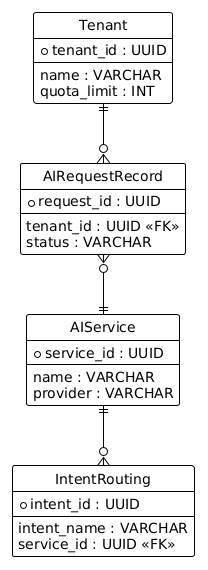
\includegraphics[width=0.35\textwidth]{images/ldm_sprint2.png}
    \caption{Logical Data Model (LDM)}
    \label{fig:ldm_sprint2}
\end{figure}

Looking at the Logical Data Model, every single \texttt{AIRequestRecord} is immutably bound to a specific \texttt{tenant\_id}. We don't just rely on application-level filtering (like adding \texttt{WHERE tenant\_id = X} to our queries), as that is prone to human error. Instead, we use Postgres Row-Level Security (RLS). This means that even if the application code had a bug, the database kernel itself physically prevents an attacker from querying records belonging to a different tenant.

\subsection{Software Design}

\subsubsection{Static View: Class Diagram}

Handling thousands of concurrent AI streams without freezing the server is a major technical challenge. To solve this, we heavily leveraged Python's \texttt{asyncio} capabilities and built the system using strict Dependency Injection.

\begin{figure}[H]
    \centering
    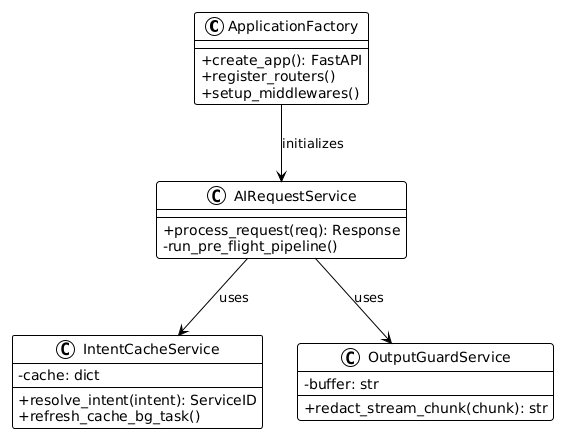
\includegraphics[width=0.85\textwidth]{images/sprint2_class.png}
    \caption{FastAPI Backend Class Diagram}
    \label{fig:sprint2_class}
\end{figure}

The class diagram above highlights the \texttt{ApplicationFactory}, which is responsible for wiring up routers and middlewares during startup. The heavy lifting is done by the \texttt{AIRequestService}. It orchestrates the flow by talking to the \texttt{IntentCacheService} (which maps user prompts to the correct LLM) and the \texttt{OutputGuardService} (which sanitizes the AI's text stream before sending it to the user).

\subsubsection{Dynamic View: End-to-End Orchestration Sequence}

To really understand how the security plugins, the routing logic, and the streaming guardrails all work together, we mapped out the complete end-to-end execution sequence. This shows the exact lifecycle of a prompt—from the moment it hits the firewall, to the moment the AI responds.

\begin{figure}[H]
    \centering
    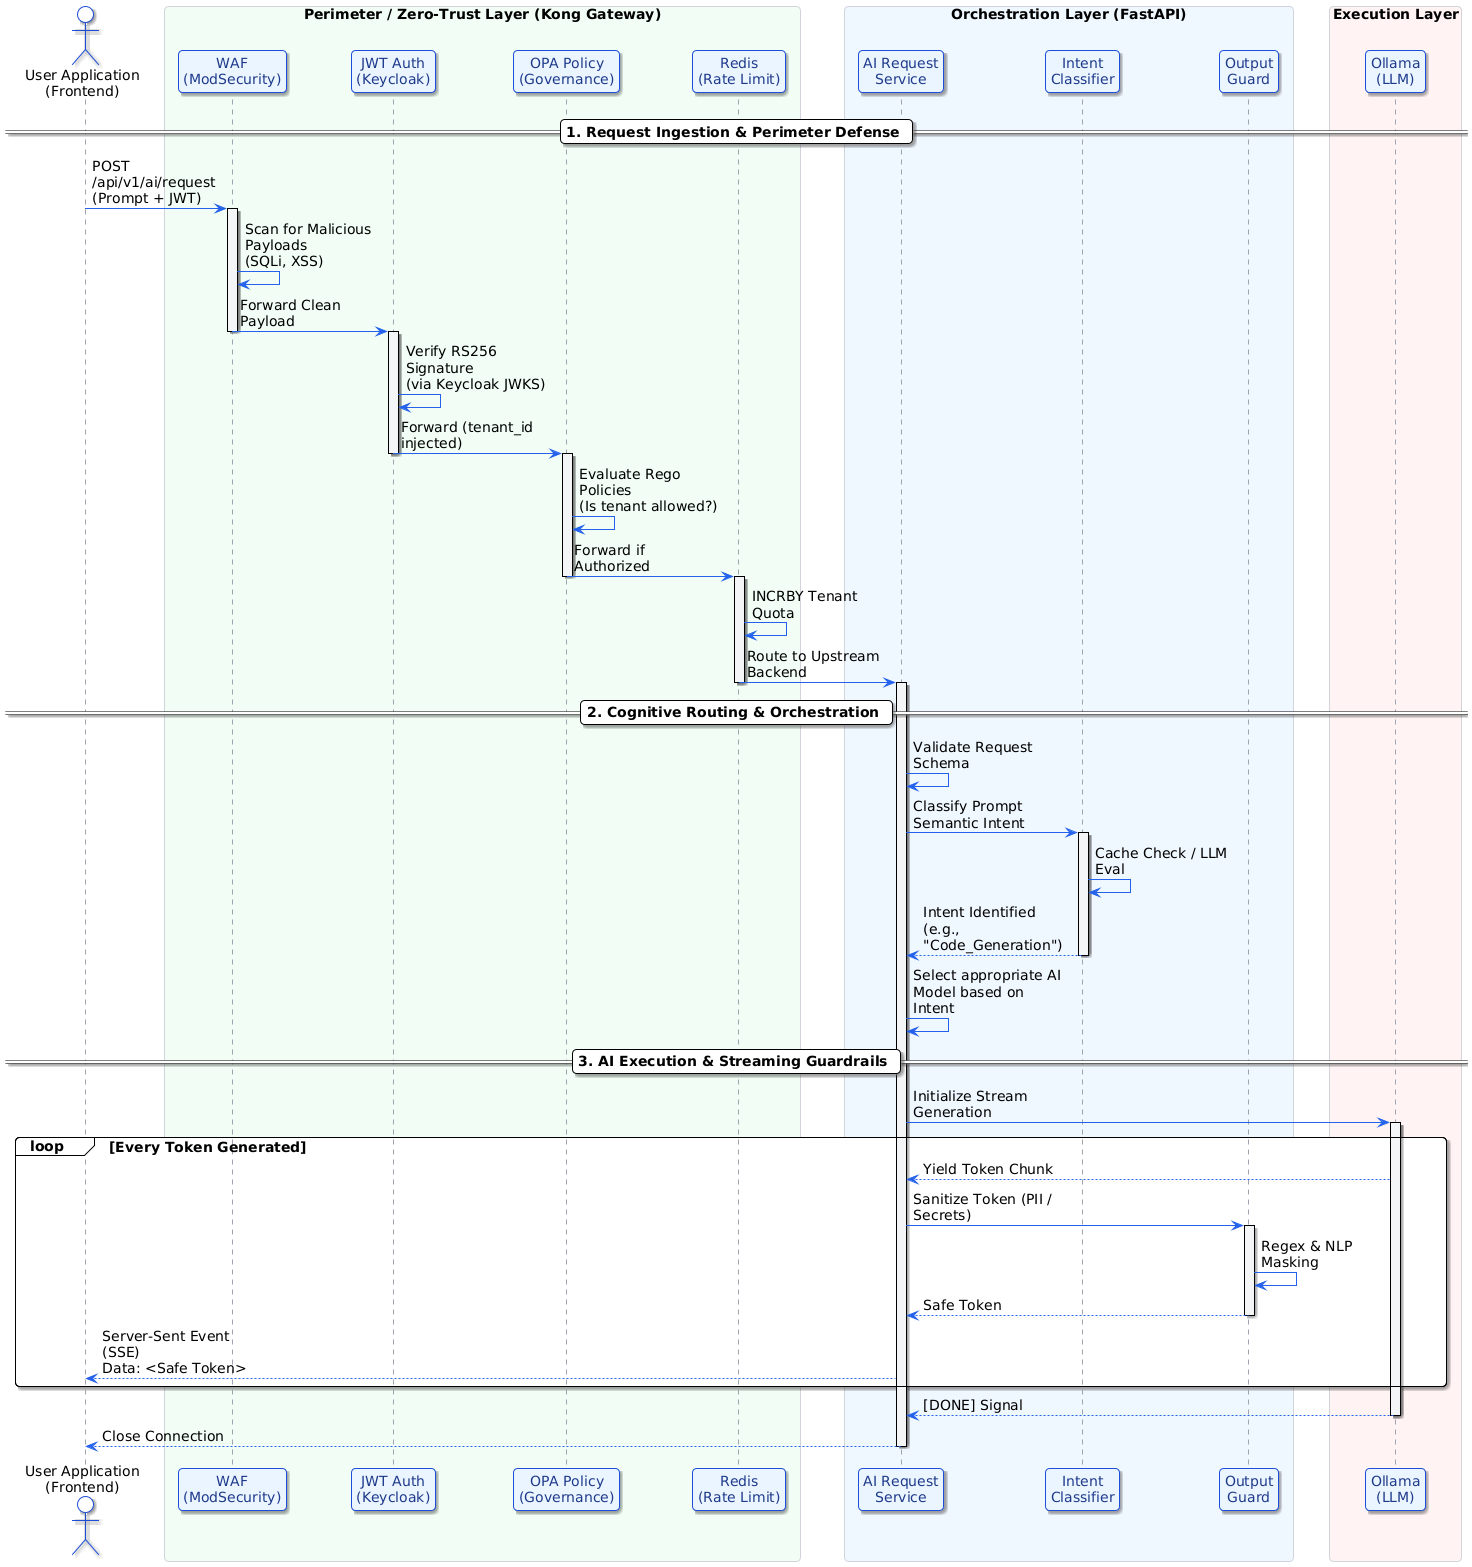
\includegraphics[width=1\textwidth]{images/end_to_end_orchestration.png}
    \caption{End-to-End AI Orchestration Sequence}
    \label{fig:end_to_end_orchestration}
\end{figure}

As mapped out in the sequence diagram, every request is governed across three distinct layers:

\begin{enumerate}
    \item \textbf{The Zero-Trust Perimeter:} The user's prompt is first scrubbed by the Web Application Firewall (WAF). It then hits Kong, where Keycloak mathematically verifies the JWT. Next, the Open Policy Agent (OPA) checks if the tenant actually has permission to make the request, and Redis verifies they haven't exceeded their API quota. If any of these checks fail, the request is killed instantly.
    \item \textbf{Cognitive Routing:} Once safely inside the backend, we don't just send the prompt to a massive monolithic LLM. Instead, the \texttt{IntentClassifier} analyzes the semantic meaning of the user's prompt (e.g., is this a coding question or a data analysis request?) and routes it to a smaller, specialized AI model that handles that specific task.
    \item \textbf{Streaming \& Guardrails:} Once the local LLM (Ollama) starts answering, it generates text word-by-word. Our backend initiates an asynchronous stream, and the \texttt{OutputGuardService} inspects every single chunk in real-time. If it detects sensitive data (like a credit card number), it redacts it before the token ever leaves the platform via Server-Sent Events (SSE).
\end{enumerate}

This architecture gives us absolute deterministic control over the entire enterprise AI workload. We've decoupled the security perimeter from the AI routing, resulting in a system that is incredibly fast, scalable, and secure.

\subsection{Showcase}
\label{subsec:sprint2_showcase}

The following figures showcase the core orchestration and real-time streaming capabilities of the platform.

\begin{figure}[H]
    \centering
    \includegraphics[width=0.85\textwidth]{images/chat_intent.png}
    \caption{AI Orchestration interface with dynamic intent classification and model routing.}
    \label{fig:chat_intent}
\end{figure}

\begin{figure}[H]
    \centering
    \includegraphics[width=0.85\textwidth]{images/ai_streaming.png}
    \caption{Low-latency AI response streaming via Server-Sent Events (SSE).}
    \label{fig:ai_streaming}
\end{figure}

\begin{figure}[H]
    \centering
    \includegraphics[width=0.85\textwidth]{images/db_audit_log.png}
    \caption{Database audit trail capturing the full request lifecycle and orchestration metadata.}
    \label{fig:db_audit_log}
\end{figure}


% ──────────────────────────────────────────────────────────────────
\section*{Conclusion}
\addcontentsline{toc}{section}{Conclusion}
% ──────────────────────────────────────────────────────────────────

In this chapter, we successfully delivered the platform's first major release. Through Sprint 1, we established a Zero-Trust security perimeter using Kong and Keycloak, ensuring that malicious or unauthenticated traffic is dropped at the network edge. In Sprint 2, we built the core FastAPI orchestration engine, enabling intelligent intent routing and real-time, token-by-token streaming. This provided us with a fully functional, highly secure foundation. In the next chapter, we will build upon this by integrating advanced governance policies, strict data quotas, and proactive security hardening.
